\subsection{Discretization of the Controller}\label{ssec:discnController}
The discretization process of a controller consists in using the map from the continuous domain to the discrete domain (z-domain), with respect to the sampling time, \si{T}, of the feedback control system:
%
\begin{flalign} 
  &\si{s = j \omega \to z = e^{s T}}\label{exp:cont2Disc}&
\end{flalign}
%
Since, by definition, the discrete domain cannot represent the complete behavior of a system through time, approximations are used to estimate this behavior.

One of the most commonly used aproximations is the bilinear transform (or Tustin's method) which is based on the trapezoidal integration principle. A reason to use this method instead of others is that it maps the entire LHP (stable area in the continuous domain) into the unit circle (stable area in the discrete domain)\cite{GFranklin}.\\
The bilinear approximation of \si{z} is defined as:
%
\begin{flalign} 
  &\si{z \approx \frac{1 + s \frac{T}{2}}{1 - s\frac{T}{2}}}\label{exp:bilinearTransform}&
\end{flalign}
%
The inverse transformation of \expr{exp:bilinearTransform} is given by:
%
\begin{flalign} 
  &\si{s \approx \frac{T}{2} \cdot \frac{1 - z^{-1}}{1 + z^{-1}}}\label{exp:inverseBilinearTransform}&
\end{flalign}
%
In general, the \expr{exp:inverseBilinearTransform} is used to replace \si{s} in the continuous-time transfer function of the designed controller. However, due to the non-linear mapping induced by the discretization, a pre-warp of the frequencies can be used before. This avoids effects of phase lag near the cross-over frequency and thus, also avoids unwanted reduction of gain and phase margins, see \cite{GGu,AVOppenheim}. 

Moreover, Matlab has an available function, \lstinline{c2d()}, designed to convert a continuous system's transfer function into the discrete domain by specifying the sampling time (here, \si{T = 0.01s}\fxnote{A justification fo this sampling time should be added at some point.}) and the desired method. The \lstinline{'prewarp'} option that is used, needs a supplementary argument corresponding to the critical fequency, chosen here to be \si{33,5\ rad \cdot s^{-1}}, see \cite{Matlabc2d}.

\Figref{fig:bodePrewarpVsNoPrewarpVsContinuous} shows Bode plots comparing the original continuous controller's frequency and phase responses with the discretized controller's with both normal Tustin's method and pre-warping, while \figref{fig:bodePrewarpVsNoPrewarpVsContinuousClosedLoop}, shows the system's closed loop responses with these controllers.\\ 
% 
\begin{minipage}{\linewidth}
  \begin{minipage}{0.45\linewidth}
    \begin{figure}[H]
      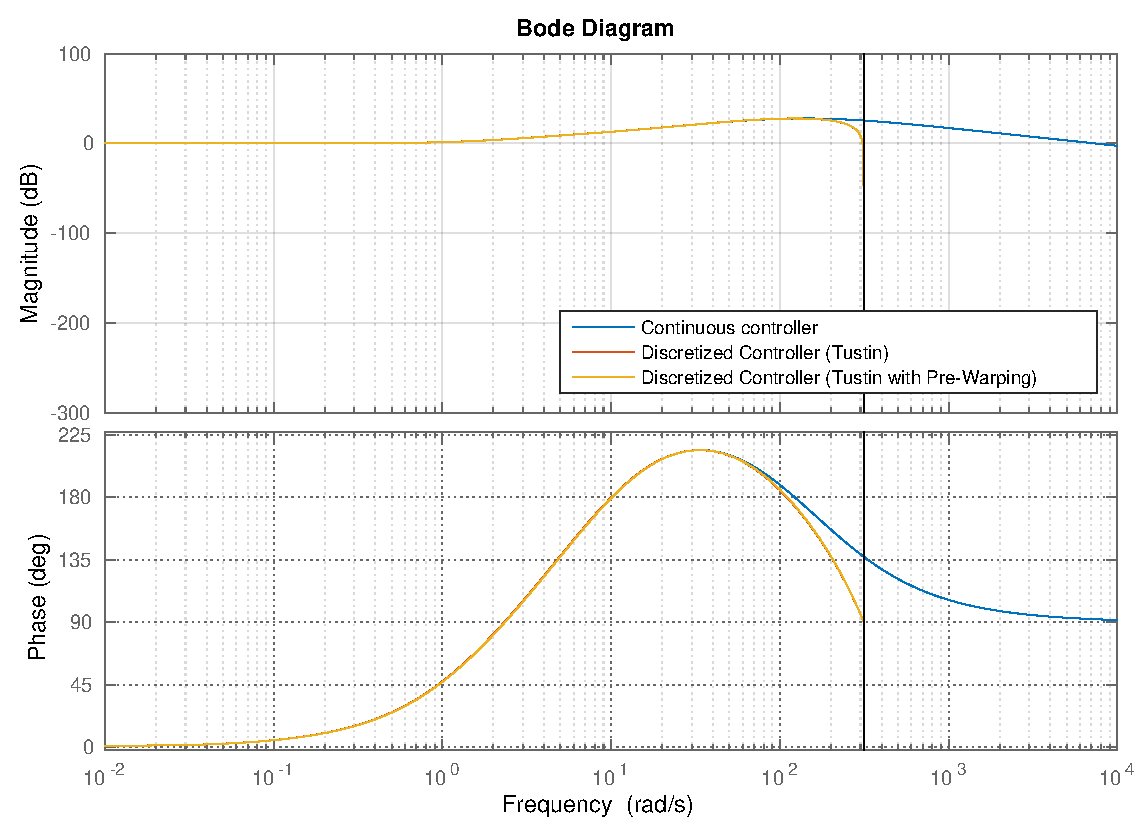
\includegraphics[scale=.4]{figures/prewarpVsNoPrewarpVsContinuousBode.pdf}
      \centering
      \captionsetup{justification=centering}
      \captionof{figure}{Bode plot of the continuous controller (in blue), discretized controller \\(in red) and pre-warped discretized controller (in orange)}
      \label{fig:bodePrewarpVsNoPrewarpVsContinuous}
    \end{figure}\vspace{-5mm}
  \end{minipage}
  \hspace{0.03\linewidth}
  \begin{minipage}{0.45\linewidth}
    \begin{figure}[H]
      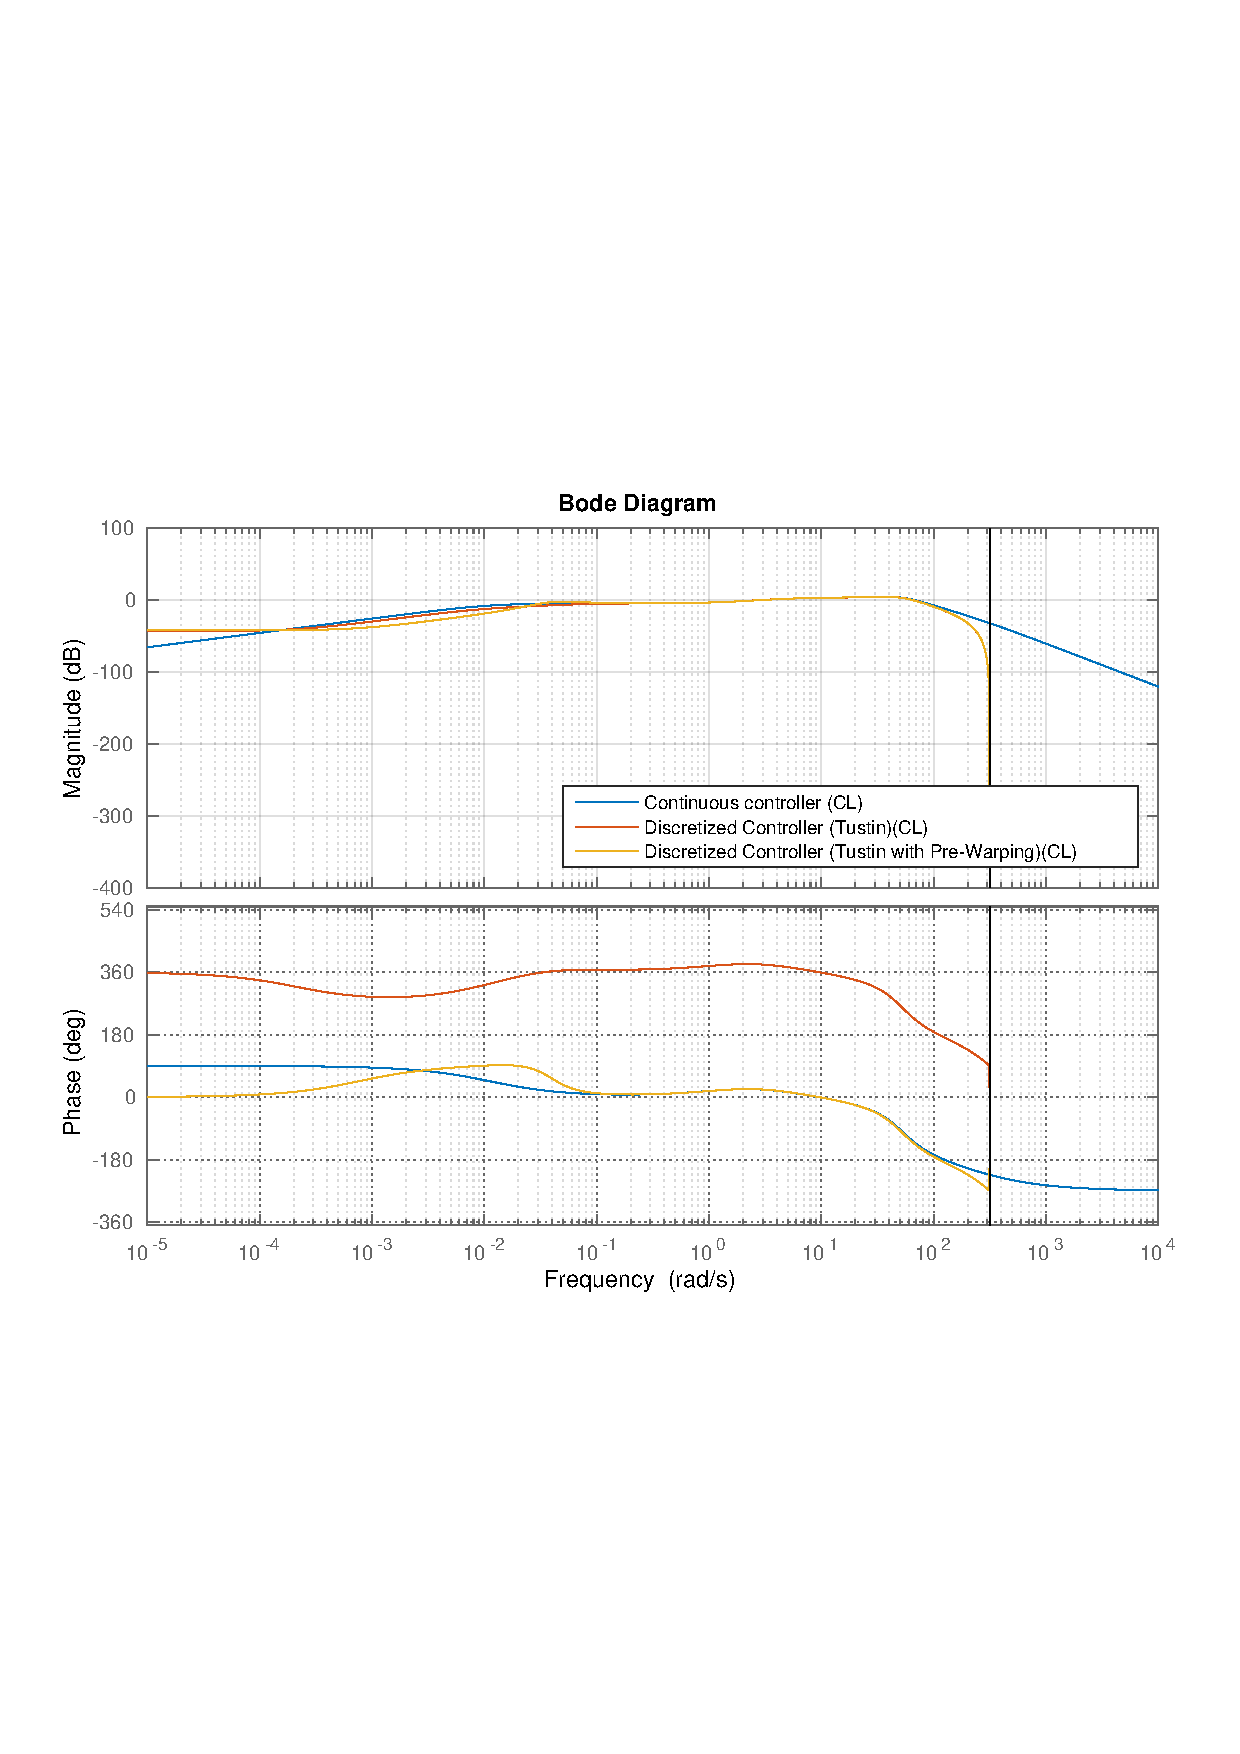
\includegraphics[scale=.4]{figures/prewarpVsNoPrewarpVsContinuousBodeClosedLoop.pdf}
      \centering
      \captionsetup{justification=centering}
      \captionof{figure}{Bode plot of the closed loop system with the continuous controller\\ (in blue), discretized controller (in red) and pre-warped discretized controller (in orange)}
      \label{fig:bodePrewarpVsNoPrewarpVsContinuousClosedLoop}
    \end{figure}\vspace{-5mm}
  \end{minipage}
\end{minipage}

From \figref{fig:bodePrewarpVsNoPrewarpVsContinuous}, it is possible to see that the discretized controllers match closely with the continuous one until approximately \si{10^{2}\ rad \cdot s^{-1}} where the phase from the discrete versions diverge from the original one. The discrete systems here, are only plotted before the vertical line which represents the Nyquist frequency, i.e. a half of the sampling frequency, chosen earlier in this section\fxnote{If the frequency choic is further explained, the corresponding section should be used as a reference here.}. More importantly, the two discrete versions of the controller, the red one using a simple Tustin method and the orange one using also pre-warping, seem very similar both in frequency and phase.

However, when looking at the second graph, on \figref{fig:bodePrewarpVsNoPrewarpVsContinuousClosedLoop}, it is apparent that the phase of the pre-warped controller follows more closely the phase of the continuous version, which is desirable. Indeed, they both align by a few degrees between \si{10^{-1}\ rad \cdot s^{-1}} and \si{10^{2}\ rad \cdot s^{-1}} and are off by \si{90^{\circ}} maximum elsewhere. On the contrary, the non-pre-warped discrete controller has a huge phase shift of close to a complete cycle (\si{360^{\circ}}) which can reveal some badly unwanted effects when running the system.

Thus, the pre-warped discretized controller is chosen for the actual implementation on the Cubli, in the code base, see \secref{sec:codeBase}, and its discrete transfer function is:
\begin{flalign}
  \eq{D(z)} {\frac{\tau_{m,w}(z)}{e_{\theta}(z)} = \frac{\num{-13,25} + \num{11,83} \cdot z^{-1} + \num{13,23} \cdot z^{-2} - \num{11,85} \cdot z^{-3}}{1 - \num{1,382} \cdot z^{-1} + \num{0,3415} \cdot z^{-2} + \num{0,001638} \cdot z^{-3}}} &%\unit{N \cdot m} 
  \label{eq:discControllerTf}
\end{flalign}
To implement a discrete controller in a code environment, the preferred form is the difference equation. This is why \eqref{eq:discControllerTf} is transformed into:
\begin{flalign}
  \eq{\tau_{m,w}[n]}{\num{-13,25} \cdot e_{\theta}[n]+ \num{11,83} \cdot e_{\theta}[n-1] + \num{13,23} \cdot e_{\theta}[n-2] - \num{11,85} \cdot e_{\theta}[n-3] + \num{1,382} \cdot \tau_{m,w}[n-1] - \num{0,3415} \cdot \tau_{m,w}[n-2] - \num{0,001638} \cdot \tau_{m,w}[n-3]}\unit{N \cdot m} 
  \label{eq:discControllerDiffEq}
\end{flalign}
\fxnote{Correct the formatting (look at the right black board or ask Niels about it).}
%
\hspace{6mm} Where:\\
\begin{tabular}{ p{1cm} l l l}
& \si{\tau_{m,w}}         & is the wanted motor torque                                          &\unitWh{N \cdot m} \\
& \si{e_{\theta}}         & is the error between wanted and measured frame angle                &\unitWh{rad}\\
& \si{x[n-m]}              & is the m-th previous state of a signal x, m = 0,1,2,3 &\unitWh{\cdot}\\
\end{tabular}

In this subsection, the designed controller has been discretized. The next subsection goes into further analysis of the new feedback control system before the actual implementation on the real system.